\documentclass[12pt]{article}
\setlength{\oddsidemargin}{0in}
\setlength{\evensidemargin}{0in}
\setlength{\textwidth}{6.5in}
\setlength{\parindent}{0in}
\setlength{\parskip}{\baselineskip}

\usepackage[letterpaper, portrait, margin=1in]{geometry}
\usepackage[usenames, dvipsnames, rgb]{xcolor}
\usepackage{amsmath,amsfonts,amssymb,circuitikz,pdfpages,tikz}

\usetikzlibrary{matrix,calc,circuits.logic.US}
\tikzstyle{branch}=[fill, shape=circle, minimum size=3pt, inner sep=0pt]

%isolated term
%#1 - Optional. Space between node and grouping line. Default=0
%#2 - node
%#3 - filling color
\newcommand{\implicantsol}[3][0]{
    \draw[rounded corners=3pt, fill=#3, opacity=0.3] ($(#2.north west)+(135:#1)$) rectangle ($(#2.south east)+(-45:#1)$);
    }


%internal group
%#1 - Optional. Space between node and grouping line. Default=0
%#2 - top left node
%#3 - bottom right node
%#4 - filling color
\newcommand{\implicant}[4][0]{
    \draw[rounded corners=3pt, fill=#4, opacity=0.3] ($(#2.north west)+(135:#1)$) rectangle ($(#3.south east)+(-45:#1)$);
    }

%group lateral borders
%#1 - Optional. Space between node and grouping line. Default=0
%#2 - top left node
%#3 - bottom right node
%#4 - filling color
\newcommand{\implicantcostats}[4][0]{
    \draw[rounded corners=3pt, fill=#4, opacity=0.3] ($(rf.east |- #2.north)+(90:#1)$)-| ($(#2.east)+(0:#1)$) |- ($(rf.east |- #3.south)+(-90:#1)$);
    \draw[rounded corners=3pt, fill=#4, opacity=0.3] ($(cf.west |- #2.north)+(90:#1)$) -| ($(#3.west)+(180:#1)$) |- ($(cf.west |- #3.south)+(-90:#1)$);
}

%group top-bottom borders
%#1 - Optional. Space between node and grouping line. Default=0
%#2 - top left node
%#3 - bottom right node
%#4 - filling color
\newcommand{\implicantdaltbaix}[4][0]{
    \draw[rounded corners=3pt, fill=#4, opacity=0.3] ($(cf.south -| #2.west)+(180:#1)$) |- ($(#2.south)+(-90:#1)$) -| ($(cf.south -| #3.east)+(0:#1)$);
    \draw[rounded corners=3pt, fill=#4, opacity=0.3] ($(rf.north -| #2.west)+(180:#1)$) |- ($(#3.north)+(90:#1)$) -| ($(rf.north -| #3.east)+(0:#1)$);
}

%group corners
%#1 - Optional. Space between node and grouping line. Default=0
%#2 - filling color
\newcommand{\implicantcantons}[2][0]{
    \draw[rounded corners=3pt, opacity=.3] ($(rf.east |- 0.south)+(-90:#1)$) -| ($(0.east |- cf.south)+(0:#1)$);
    \draw[rounded corners=3pt, opacity=.3] ($(rf.east |- 8.north)+(90:#1)$) -| ($(8.east |- rf.north)+(0:#1)$);
    \draw[rounded corners=3pt, opacity=.3] ($(cf.west |- 2.south)+(-90:#1)$) -| ($(2.west |- cf.south)+(180:#1)$);
    \draw[rounded corners=3pt, opacity=.3] ($(cf.west |- 10.north)+(90:#1)$) -| ($(10.west |- rf.north)+(180:#1)$);
    \fill[rounded corners=3pt, fill=#2, opacity=.3] ($(rf.east |- 0.south)+(-90:#1)$) -|  ($(0.east |- cf.south)+(0:#1)$) [sharp corners] ($(rf.east |- 0.south)+(-90:#1)$) |-  ($(0.east |- cf.south)+(0:#1)$) ;
    \fill[rounded corners=3pt, fill=#2, opacity=.3] ($(rf.east |- 8.north)+(90:#1)$) -| ($(8.east |- rf.north)+(0:#1)$) [sharp corners] ($(rf.east |- 8.north)+(90:#1)$) |- ($(8.east |- rf.north)+(0:#1)$) ;
    \fill[rounded corners=3pt, fill=#2, opacity=.3] ($(cf.west |- 2.south)+(-90:#1)$) -| ($(2.west |- cf.south)+(180:#1)$) [sharp corners]($(cf.west |- 2.south)+(-90:#1)$) |- ($(2.west |- cf.south)+(180:#1)$) ;
    \fill[rounded corners=3pt, fill=#2, opacity=.3] ($(cf.west |- 10.north)+(90:#1)$) -| ($(10.west |- rf.north)+(180:#1)$) [sharp corners] ($(cf.west |- 10.north)+(90:#1)$) |- ($(10.west |- rf.north)+(180:#1)$) ;
}

%Empty Karnaugh map 4x4
\newenvironment{Karnaugh}%
{
\begin{tikzpicture}[baseline=(current bounding box.north),scale=0.8]
\draw (0,0) grid (4,4);
\draw (0,4) -- node [pos=1,above right,anchor=south west] {$x_3x_4$} node [pos=0.7,below left,anchor=north east] {$x_1x_2$} ++(135:1);
%
\matrix (mapa) [matrix of nodes,
        column sep={0.8cm,between origins},
        row sep={0.8cm,between origins},
        every node/.style={minimum size=0.3mm},
        anchor=8.center,
        ampersand replacement=\&] at (0.5,0.5)
{
                       \& |(c00)| 00         \& |(c01)| 01         \& |(c11)| 11         \& |(c10)| 10         \& |(cf)| \phantom{00} \\
|(r00)| 00             \& |(0)|  \phantom{0} \& |(1)|  \phantom{0} \& |(3)|  \phantom{0} \& |(2)|  \phantom{0} \&                     \\
|(r01)| 01             \& |(4)|  \phantom{0} \& |(5)|  \phantom{0} \& |(7)|  \phantom{0} \& |(6)|  \phantom{0} \&                     \\
|(r11)| 11             \& |(12)| \phantom{0} \& |(13)| \phantom{0} \& |(15)| \phantom{0} \& |(14)| \phantom{0} \&                     \\
|(r10)| 10             \& |(8)|  \phantom{0} \& |(9)|  \phantom{0} \& |(11)| \phantom{0} \& |(10)| \phantom{0} \&                     \\
|(rf) | \phantom{00}   \&                    \&                    \&                    \&                    \&                     \\
};
}%
{
\end{tikzpicture}
}

%Empty Karnaugh map 4x4
\newenvironment{Karnaugh5}%
{
\begin{tikzpicture}[baseline=(current bounding box.north),scale=0.8]
\draw (0,0) grid (4,4);
\draw (0,4) -- node [pos=1,above right,anchor=south west] {$x_4x_5$} node [pos=0.7,below left,anchor=north east] {$x_2x_3$} ++(135:1);
%
\matrix (mapa) [matrix of nodes,
        column sep={0.8cm,between origins},
        row sep={0.8cm,between origins},
        every node/.style={minimum size=0.3mm},
        anchor=8.center,
        ampersand replacement=\&] at (0.5,0.5)
{
                       \& |(c00)| 00         \& |(c01)| 01         \& |(c11)| 11         \& |(c10)| 10         \& |(cf)| \phantom{00} \\
|(r00)| 00             \& |(0)|  \phantom{0} \& |(1)|  \phantom{0} \& |(3)|  \phantom{0} \& |(2)|  \phantom{0} \&                     \\
|(r01)| 01             \& |(4)|  \phantom{0} \& |(5)|  \phantom{0} \& |(7)|  \phantom{0} \& |(6)|  \phantom{0} \&                     \\
|(r11)| 11             \& |(12)| \phantom{0} \& |(13)| \phantom{0} \& |(15)| \phantom{0} \& |(14)| \phantom{0} \&                     \\
|(r10)| 10             \& |(8)|  \phantom{0} \& |(9)|  \phantom{0} \& |(11)| \phantom{0} \& |(10)| \phantom{0} \&                     \\
|(rf) | \phantom{00}   \&                    \&                    \&                    \&                    \&                     \\
};
}%
{
\end{tikzpicture}
}

%Empty Karnaugh map 2x4
\newenvironment{Karnaughvuit}%
{
\begin{tikzpicture}[baseline=(current bounding box.north),scale=0.8]
\draw (0,0) grid (4,2);
\draw (0,2) -- node [pos=1,above right,anchor=south west] {$x_2x_3$} node [pos=0.7,below left,anchor=north east] {$x_1$} ++(135:1);
%
\matrix (mapa) [matrix of nodes,
        column sep={0.8cm,between origins},
        row sep={0.8cm,between origins},
        every node/.style={minimum size=0.3mm},
        anchor=4.center,
        ampersand replacement=\&] at (0.5,0.5)
{
                      \& |(c00)| 00         \& |(c01)| 01         \& |(c11)| 11         \& |(c10)| 10         \& |(cf)| \phantom{00} \\
|(r00)| 0             \& |(0)|  \phantom{0} \& |(1)|  \phantom{0} \& |(3)|  \phantom{0} \& |(2)|  \phantom{0} \&                     \\
|(r01)| 1             \& |(4)|  \phantom{0} \& |(5)|  \phantom{0} \& |(7)|  \phantom{0} \& |(6)|  \phantom{0} \&                     \\
|(rf) | \phantom{00}  \&                    \&                    \&                    \&                    \&                     \\
};
}%
{
\end{tikzpicture}
}

%Empty Karnaugh map 2x2
\newenvironment{Karnaughquatre}%
{
\begin{tikzpicture}[baseline=(current bounding box.north),scale=0.8]
\draw (0,0) grid (2,2);
\draw (0,2) -- node [pos=0.7,above right,anchor=south west] {b} node [pos=0.7,below left,anchor=north east] {a} ++(135:1);
%
\matrix (mapa) [matrix of nodes,
        column sep={0.8cm,between origins},
        row sep={0.8cm,between origins},
        every node/.style={minimum size=0.3mm},
        anchor=2.center,
        ampersand replacement=\&] at (0.5,0.5)
{
          \& |(c00)| 0          \& |(c01)| 1  \\
|(r00)| 0 \& |(0)|  \phantom{0} \& |(1)|  \phantom{0} \\
|(r01)| 1 \& |(2)|  \phantom{0} \& |(3)|  \phantom{0} \\
};
}%
{
\end{tikzpicture}
}

%Defines 8 or 16 values (0,1,X)
\newcommand{\contingut}[1]{%
\foreach \x [count=\xi from 0]  in {#1}
     \path (\xi) node {\x};
}

%Places 1 in listed positions
\newcommand{\minterms}[1]{%
    \foreach \x in {#1}
        \path (\x) node {1};
}

%Places 0 in listed positions
\newcommand{\maxterms}[1]{%
    \foreach \x in {#1}
        \path (\x) node {0};
}

\newcommand{\overbar}[1]{\mkern 1.5mu\overline{\mkern-1.5mu#1\mkern-1.5mu}\mkern 1.5mu}

\begin{document}
\title{Digital Logic Homework 4}

ECEN 2350 Spring 2017 \hfill Homework 4\\
Samuel Cuthbertson

\hrulefill

\begin{enumerate}
	\vspace{-4mm}
	\item \textit{Book Problems: 2.77 and 2.78}
	      \begin{enumerate}

	      	\item[(2.77)] \textit{What is the cost of the circuit shown in the book, assuming the input variables are available in both true and complemented forms? Redesign the circuit to implement the same functions, but at as low a cost as possible. What is the cost of your circuit?}

	      	      Noting that the circuit can be expressed as the logic equations:
	      	      \begin{align*}
	      	      	f & = \overbar{(x_1+x_3+x_4)} + x_4(x_1+x_3) + \overbar{x_1}\overbar{x_2}x_3 + x_1x_2\overbar{x_3}\overbar{x_4}    \\
	      	      	g & = x_1x_2\overbar{x_3}\overbar{x_4} + \overbar{x_2}x_4 + x_3(\overbar{x_1}+\overbar{x_4}) + \overbar{(x_1+x_4)}
	      	      \end{align*}
	      	      Which, noting that $x_1x_2\overbar{x_3}\overbar{x_4}$ is in both equations and only in the circuit once, as well as assuming that the complemented form of each variable is available for free, has the cost of $\left((1+2+1+1)+1\right) + \left((1+2+1)+1\right)=6+5=11$ gates and $\left((3+(2+2)+3+4)+4\right) + \left((2+(2+2)+2)+4\right) = 18 + 12 = 30$ inputs. Total cost is then $30+11 = \boxed{41}$ \\
	      	      Additionally, the logic equations above can be expanded into:
	      	      \begin{align*}
	      	      	f & = \overbar{x_1}\overbar{x_3}\overbar{x_4} + x_4x_1 + x_4x_3 + \overbar{x_1}\overbar{x_2}x_3 + x_1x_2\overbar{x_3}\overbar{x_4} &   & \textit{Distributive, DeMorgan's} \\
	      	      	g & = x_1x_2\overbar{x_3}\overbar{x_4} + \overbar{x_2}x_4 + x_3\overbar{x_1}+x_3\overbar{x_4} + \overbar{x_1}\overbar{x_4}         &   & \textit{Distributive, DeMorgan's}
	      	      \end{align*}
	      	      \begin{center}
	      	      	\begin{minipage}{0.4\textwidth}
	      	      		\begin{center}
	      	      			\[
	      	      				f = \color{magenta}{\overbar{x_1}\overbar{x_3}\overbar{x_4}} \color{black}{+} \color{blue}{x_4x_1} \color{black}{+} \color{red}{x_4x_3} \color{black}{+} \color{orange}{\overbar{x_1}\overbar{x_2}x_3} \color{black}{+} \color{cyan}{x_1x_2\overbar{x_3}\overbar{x_4}}
	      	      			\]
	      	      			\begin{Karnaugh}
	      	      				\contingut{1,0,1,1,1,0,0,1,0,1,0,1,1,1,0,1}
	      	      				\implicantsol{12}{cyan}
	      	      				\implicant{3}{2}{orange}
	      	      				\implicant{3}{11}{red}
	      	      				\implicant{13}{11}{blue}
	      	      				\implicant{0}{4}{magenta}
	      	      			\end{Karnaugh}
	      	      		\end{center}
	      	      	\end{minipage}
	      	      	\hfill
	      	      	\begin{minipage}{0.4\textwidth}
	      	      		\begin{center}
	      	      			\begin{Karnaugh}
	      	      				\contingut{1,1,1,1,1,0,1,1,0,1,1,1,1,0,1,0}
	      	      				\implicantsol{12}{cyan}
	      	      				\implicantdaltbaix{1}{11}{orange}
	      	      				\implicant{3}{6}{red}
	      	      				\implicantcostats{0}{6}{magenta}
	      	      				\implicant{2}{10}{blue}
	      	      			\end{Karnaugh}
	      	      			\[
	      	      				g = \color{cyan}{x_1x_2\overbar{x_3}\overbar{x_4}} \color{black}{+} \color{orange}{\overbar{x_2}x_4} \color{black}{+} \color{red}{x_3\overbar{x_1}} \color{black}{+} \color{blue}{x_3\overbar{x_4}} \color{black}{+} \color{magenta}{\overbar{x_1}\overbar{x_4}}
	      	      			\]
	      	      		\end{center}
	      	      	\end{minipage}
	      	      	Maximizing shared terms, we can further simplify the above into:\\
	      	      	\begin{minipage}{0.4\textwidth}
	      	      		\begin{center}
	      	      			\[
	      	      				f = \color{magenta}{\overbar{x_1}\overbar{x_2}\overbar{x_4}} \color{black}{+} \color{blue}{x_4x_1} \color{black}{+} \color{red}{\overbar{x_1}x_3x_4} \color{black}{+} \color{cyan}{x_2\overbar{x_3}\overbar{x_4}}
	      	      			\]
	      	      			\begin{Karnaugh}
	      	      				\contingut{1,0,1,1,1,0,0,1,0,1,0,1,1,1,0,1}
	      	      				\implicant{4}{12}{cyan}
	      	      				\implicant{3}{7}{red}
	      	      				\implicant{13}{11}{blue}
	      	      				\implicantcostats{0}{2}{magenta}
	      	      			\end{Karnaugh}
	      	      		\end{center}
	      	      	\end{minipage}
	      	      	\hfill
	      	      	\begin{minipage}{0.4\textwidth}
	      	      		\begin{center}
	      	      			\begin{Karnaugh}
	      	      				\contingut{1,1,1,1,1,0,1,1,0,1,1,1,1,0,1,0}
	      	      				\implicant{4}{12}{cyan}
	      	      				\implicantdaltbaix{1}{11}{orange}
	      	      				\implicant{3}{7}{red}
	      	      				\implicantcostats{0}{2}{magenta}
	      	      				\implicant{2}{10}{blue}
	      	      			\end{Karnaugh}
	      	      			\[
	      	      				g = \color{magenta}{\overbar{x_1}\overbar{x_2}\overbar{x_4}} \color{black}{+} \color{blue}{x_3\overbar{x_4}} \color{black}{+} \color{red}{\overbar{x_1}x_3x_4} \color{black}{+} \color{cyan}{x_2\overbar{x_3}\overbar{x_4}} \color{black}{+} \color{orange}{\overbar{x_1}\overbar{x_2}x_4}
	      	      			\]
	      	      		\end{center}
	      	      	\end{minipage}
	      	      \end{center}
	      	      The above equations share terms $\overbar{x_1}\overbar{x_2}\overbar{x_4}$, $\overbar{x_1}x_3x_4$, $x_2\overbar{x_3}\overbar{x_4}$. They can also be simplified further:
	      	      \begin{align*}
	      	      	f & = \color{magenta}{\overbar{x_1}\overbar{x_2}\overbar{x_4}} \color{black}{+} \color{blue}{x_4x_1} \color{black}{+} \color{red}{\overbar{x_1}x_3x_4} \color{black}{+} \color{cyan}{x_2\overbar{x_3}\overbar{x_4}}                                                                          \\
	      	      	g & = \color{magenta}{\overbar{x_1}\overbar{x_2}\overbar{x_4}} \color{black}{+} \color{blue}{x_3\overbar{x_4}} \color{black}{+} \color{red}{\overbar{x_1}x_3x_4} \color{black}{+} \color{cyan}{x_2\overbar{x_3}\overbar{x_4}} \color{black}{+} \color{orange}{\overbar{x_1}\overbar{x_2}x_4}
	      	      \end{align*}

	      	      Thus the cost of the circuit would be $\left((1+1+1+1)+1\right)+\left((1+1)+1\right) = 5 + 3 = 8$ gates and $\left((3+2+3+3)+4\right) + \left((2+3)+5\right) = 15 + 10 = 25$ inputs, for a total cost of $8+25=\boxed{33}$

	      	      \begin{center}
	      	      	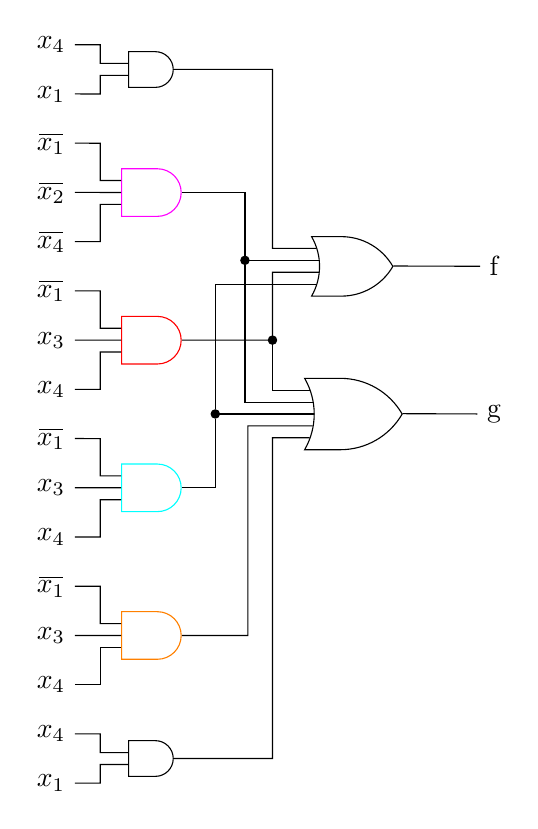
\begin{tikzpicture}[circuit logic US,scale=1.25]
	      	      		\node (aaa) at (0, 6.5) {$x_4$};
	      	      		\node (aab) at (0, 6) {$x_1$};
	      	      		\node[and gate US, draw, logic gate inputs=nn] at (1,6.25) (aag) {};
	      	      		\draw (aaa)-- ($(aaa) + (0.5,0)$)|- (aag.input 1);
	      	      		\draw (aab)-- ($(aab) + (0.5,0)$)|- (aag.input 2);

	      	      		\node (aba) at (0, 5.5) {$\overbar{x_1}$};
	      	      		\node (abb) at (0, 5) {$\overbar{x_2}$};
	      	      		\node (abc) at (0, 4.5) {$\overbar{x_4}$};
	      	      		\node[and gate US, draw, rotate=0, logic gate inputs=nnn, draw=magenta] at (1,5) (abg) {};
	      	      		\draw (aba)-- ($(aba) + (0.5,0)$)|- (abg.input 1);
	      	      		\draw (abb)-- ($(abb) + (0.5,0)$)|- (abg.input 2);
	      	      		\draw (abc)-- ($(abc) + (0.5,0)$)|- (abg.input 3);

	      	      		\node (aca) at (0, 4) {$\overbar{x_1}$};
	      	      		\node (acb) at (0, 3.5) {$x_3$};
	      	      		\node (acc) at (0, 3) {$x_4$};
	      	      		\node[and gate US, draw, rotate=0, logic gate inputs=nnn, draw=red] at (1,3.5) (acg) {};
	      	      		\draw (aca)-- ($(aca) + (0.5,0)$)|- (acg.input 1);
	      	      		\draw (acb)-- ($(acb) + (0.5,0)$)|- (acg.input 2);
	      	      		\draw (acc)-- ($(acc) + (0.5,0)$)|- (acg.input 3);

	      	      		\node (ada) at (0, 2.5) {$\overbar{x_1}$};
	      	      		\node (adb) at (0, 2) {$x_3$};
	      	      		\node (adc) at (0, 1.5) {$x_4$};
	      	      		\node[and gate US, draw, rotate=0, logic gate inputs=nnn, draw=cyan] at (1,2) (adg) {};
	      	      		\draw (ada)-- ($(ada) + (0.5,0)$)|- (adg.input 1);
	      	      		\draw (adb)-- ($(adb) + (0.5,0)$)|- (adg.input 2);
	      	      		\draw (adc)-- ($(adc) + (0.5,0)$)|- (adg.input 3);

	      	      		\node (aea) at (0, 1) {$\overbar{x_1}$};
	      	      		\node (aeb) at (0, .5) {$x_3$};
	      	      		\node (aec) at (0, 0) {$x_4$};
	      	      		\node[and gate US, draw, rotate=0, logic gate inputs=nnn, draw=orange] at (1,.5) (aeg) {};
	      	      		\draw (aea)-- ($(aea) + (0.5,0)$)|- (aeg.input 1);
	      	      		\draw (aeb)-- ($(aeb) + (0.5,0)$)|- (aeg.input 2);
	      	      		\draw (aec)-- ($(aec) + (0.5,0)$)|- (aeg.input 3);

	      	      		\node (afa) at (0, -.5) {$x_4$};
	      	      		\node (afb) at (0, -1) {$x_1$};
	      	      		\node[and gate US, draw, logic gate inputs=nn] at (1,-.75) (afg) {};
	      	      		\draw (afa)-- ($(afa) + (0.5,0)$)|- (afg.input 1);
	      	      		\draw (afb)-- ($(afb) + (0.5,0)$)|- (afg.input 2);

	      	      		%layer 2
	      	      		\node[or gate US, draw, logic gate inputs=nnnn] at (3,4.25) (orf) {};
	      	      		\node[or gate US, draw, logic gate inputs=nnnnn] at (3,2.75) (org) {};

	      	      		\draw (aag) -- ($(aag) + (1.25,0)$)|- (orf.input 1);
	      	      		\draw (acg) -- ($(acg) + (1.25,0)$)|- (orf.input 3);
	      	      		\node[branch, draw] at ($(acg) + (1.25,0)$) (acbr) {};
	      	      		\node[branch, draw] at ($(orf.input 2) - (0.75,0)$) (abbr) {};
	      	      		\draw (abg) -| (abbr) |- (orf.input 2);

	      	      		\draw (abbr)|- (org.input 2);
	      	      		\draw (acbr)|- (org.input 1);
	      	      		\node[branch, draw] at ($(org.input 3) - (1,0)$) (adbr) {};
	      	      		\draw (adg) -| (adbr) |- (org.input 3);
	      	      		\draw (adbr) |- (orf.input 4);
	      	      		\draw (aeg) -- ($(aeg) + (1,0)$)|- (org.input 4);
	      	      		\draw (afg) -- ($(afg) + (1.25,0)$)|- (org.input 5);

	      	      		%layer 4
	      	      		\node (f) at (4.5,4.25) {f};
	      	      		\node (g) at (4.5,2.75) {g};

	      	      		\draw (org) -- (g);
	      	      		\draw (orf) -- (f);

	      	      	\end{tikzpicture}
	      	      \end{center}

	      	      \newpage
	      	\item[(2.78)] \textit{What is the cost of the circuit shown in the book, assuming the input variables are available in both true and complemented forms? Redesign the circuit to implement the same functions, but at as low a cost as possible still using only NAND gates. What is the cost of your circuit?}

	      	      Noting that the circuit can be expressed as the logic equations:
	      	      \begin{align*}
	      	      	f & = x_1\overbar{x_2} + \overbar{x_1}(x_2 \otimes x_3) + \overbar{x_2}x_4                \\
	      	      	g & = \overbar{x_2}x_3 + \overbar{x_1}x_3 + \overbar{x_1}\overbar{x_2} + \overbar{x_2}x_4
	      	      \end{align*}
	      	      Which can be examined in the below K-Maps:

	      	      \begin{minipage}{0.4\textwidth}
	      	      	\begin{center}
	      	      		\[
	      	      			f = \color{blue}{x_1\overbar{x_2}} \color{black}{+} \color{cyan}{\overbar{x_1}(x_2 \otimes x_3)} \color{black}{+} \color{green}{\overbar{x_2}x_4}
	      	      		\]
	      	      		\begin{Karnaugh}
	      	      			\contingut{1,1,0,1,0,0,1,1,1,1,1,1,0,0,0,0}
	      	      			\implicant{8}{10}{blue}
	      	      			\implicantdaltbaix{1}{11}{green}
	      	      			\implicant{0}{1}{cyan}
	      	      			\implicant{7}{6}{cyan}
	      	      		\end{Karnaugh}
	      	      	\end{center}
	      	      \end{minipage}
	      	      \hfill
	      	      \begin{minipage}{0.4\textwidth}
	      	      	\begin{center}
	      	      		\begin{Karnaugh}
	      	      			\contingut{1,1,1,1,0,0,1,1,0,1,1,1,0,0,0,0}
	      	      			\implicantdaltbaix{3}{10}{green}
	      	      			\implicant{7}{6}{cyan}
	      	      			\implicant{0}{2}{orange}
	      	      			\implicant{9}{11}{red}
	      	      		\end{Karnaugh}
	      	      		\[
	      	      			g = \color{green}{\overbar{x_2}x_3} \color{black}{+} \color{cyan}{\overbar{x_1}x_3} \color{black}{+} \color{orange}{\overbar{x_1}\overbar{x_2}} \color{black}{+} \color{red}{\overbar{x_2}x_4}
	      	      		\]
	      	      	\end{center}
	      	      \end{minipage}
	      	      Simplifying the above maps into optimal covers, we see:

	      	      \begin{minipage}{0.4\textwidth}
	      	      	\begin{center}
	      	      		\begin{align*}
	      	      			f & = \color{orange}{(\overbar{x_2}+\overbar{x_2})}\color{red}{(\overbar{x_2}+x_3)}\color{Maroon}{(x_1 + x_2 + \overbar{x_3} + x_4)}                                                                      \\
	      	      			f & = \color{blue}{\overbar{x_2}x_4} \color{black}{+} \color{cyan}{\overbar{x_1}x_2x_3} \color{black}{+} \color{ForestGreen}{x_1\overbar{x_2}x_3} \color{black}{+} \color{SkyBlue}{\overbar{x_2}\overbar{x_3}}
	      	      		\end{align*}
	      	      		\begin{Karnaugh}
	      	      			\contingut{1,1,0,1,0,0,1,1,1,1,1,1,0,0,0,0}
	      	      			\implicant{4}{13}{red}
	      	      			\implicant{12}{14}{orange}
	      	      			\implicantsol{2}{Maroon}

	      	      			\implicantdaltbaix{1}{11}{blue}
	      	      			\implicant{7}{6}{cyan}
	      	      			\implicant{11}{10}{ForestGreen}
	      	      			\implicantdaltbaix{0}{9}{SkyBlue}
	      	      		\end{Karnaugh}
	      	      	\end{center}
	      	      \end{minipage}
	      	      \hfill
	      	      \begin{minipage}{0.4\textwidth}
	      	      	\begin{center}
	      	      		\begin{Karnaugh}
	      	      			\contingut{1,1,1,1,0,0,1,1,0,1,1,1,0,0,0,0}
	      	      			\implicant{4}{13}{red}
	      	      			\implicant{12}{14}{orange}
	      	      			\implicant{12}{8}{Maroon}

	      	      			\implicantdaltbaix{1}{11}{blue}
	      	      			\implicant{7}{6}{cyan}
	      	      			\implicant{11}{10}{ForestGreen}
	      	      			\implicant{0}{2}{Plum}
	      	      		\end{Karnaugh}
	      	      		\begin{align*}
	      	      			g & = \color{orange}{(\overbar{x_1}+\overbar{x_2})}\color{red}{(\overbar{x_2}+x_3)}\color{Maroon}{(\overbar{x_1} + x_3 + x_4)}                                                                           \\
	      	      			g & = \color{blue}{\overbar{x_2}x_4} \color{black}{+} \color{cyan}{\overbar{x_1}x_2x_3} \color{black}{+} \color{ForestGreen}{x_1\overbar{x_2}x_3} \color{black}{+} \color{Plum}{\overbar{x_1}\overbar{x_2}}
	      	      		\end{align*}
	      	      	\end{center}
	      	      \end{minipage}
	      	      And in analayzing the cost:
	      	      \begin{align*}
	      	      	POS & = \text{Gates} + \text{Inputs} = (3+1+1+1) + (2+2+4+3+3+3) = 23     \\
	      	      	SOP & = \text{Gates} + \text{Inputs} = (4+1+1+1) + (2+3+3+2+2+4+4) = 27
	      	      \end{align*}
	      	      However, SOP has zero additional cost in converting to NANDs while this POS will have at least an addition of 6, as each output (f and g) will have to be inverted and a NAND inverter has cost 3 (2 inputs, 1 gate). Therefor, as $23+6 = 29 > 27$ SOP is the cheapest option for NAND implementation.

                Also noting that the SOP equations can be manipulated into NANDs as follows:
                \begin{align*}
	      	      	f & = \color{blue}{\overbar{x_2}x_4} \color{black}{+} \color{cyan}{\overbar{x_1}x_2x_3} \color{black}{+} \color{ForestGreen}{x_1\overbar{x_2}x_3} \color{black}{+} \color{SkyBlue}{\overbar{x_2}\overbar{x_3}} \\
                  g & = \color{blue}{\overbar{x_2}x_4} \color{black}{+} \color{cyan}{\overbar{x_1}x_2x_3} \color{black}{+} \color{ForestGreen}{x_1\overbar{x_2}x_3} \color{black}{+} \color{Plum}{\overbar{x_1}\overbar{x_2}} \\
                \end{align*}
	      	      The circuit is shown below:
                \begin{center}
                  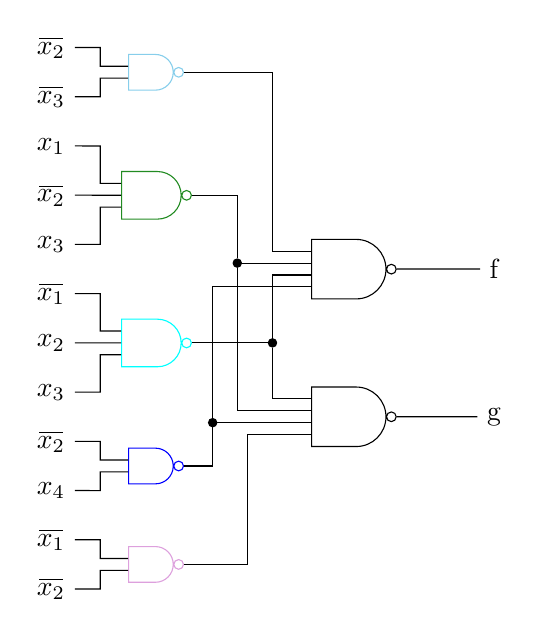
\begin{tikzpicture}[circuit logic US,scale=1.25]
                    \node (aaa) at (0, 6.5) {$\overbar{x_2}$};
                    \node (aab) at (0, 6) {$\overbar{x_3}$};
                    \node[nand gate US, draw, logic gate inputs=nn, draw=SkyBlue] at (1,6.25) (aag) {};
                    \draw (aaa)-- ($(aaa) + (0.5,0)$)|- (aag.input 1);
                    \draw (aab)-- ($(aab) + (0.5,0)$)|- (aag.input 2);

                    \node (aba) at (0, 5.5) {$x_1$};
                    \node (abb) at (0, 5) {$\overbar{x_2}$};
                    \node (abc) at (0, 4.5) {$x_3$};
                    \node[nand gate US, draw, rotate=0, logic gate inputs=nnn, draw=ForestGreen] at (1,5) (abg) {};
                    \draw (aba)-- ($(aba) + (0.5,0)$)|- (abg.input 1);
                    \draw (abb)-- ($(abb) + (0.5,0)$)|- (abg.input 2);
                    \draw (abc)-- ($(abc) + (0.5,0)$)|- (abg.input 3);

                    \node (aca) at (0, 4) {$\overbar{x_1}$};
                    \node (acb) at (0, 3.5) {$x_2$};
                    \node (acc) at (0, 3) {$x_3$};
                    \node[nand gate US, draw, rotate=0, logic gate inputs=nnn, draw=cyan] at (1,3.5) (acg) {};
                    \draw (aca)-- ($(aca) + (0.5,0)$)|- (acg.input 1);
                    \draw (acb)-- ($(acb) + (0.5,0)$)|- (acg.input 2);
                    \draw (acc)-- ($(acc) + (0.5,0)$)|- (acg.input 3);

                    \node (ada) at (0, 2.5) {$\overbar{x_2}$};
                    \node (adb) at (0, 2) {$x_4$};
                    \node[nand gate US, draw, rotate=0, logic gate inputs=nn, draw=blue] at (1,2.25) (adg) {};
                    \draw (ada)-- ($(ada) + (0.5,0)$)|- (adg.input 1);
                    \draw (adb)-- ($(adb) + (0.5,0)$)|- (adg.input 2);

                    \node (aea) at (0, 1.5) {$\overbar{x_1}$};
                    \node (aeb) at (0, 1) {$\overbar{x_2}$};
                    \node[nand gate US, draw, rotate=0, logic gate inputs=nn, draw=Plum] at (1,1.25) (aeg) {};
                    \draw (aea)-- ($(aea) + (0.5,0)$)|- (aeg.input 1);
                    \draw (aeb)-- ($(aeb) + (0.5,0)$)|- (aeg.input 2);

                    %layer 2
                    \node[nand gate US, draw, logic gate inputs=nnnn] at (3,4.25) (orf) {};
                    \node[nand gate US, draw, logic gate inputs=nnnn] at (3,2.75) (org) {};

                    \draw (aag.output) -- ($(aag) + (1.25,0)$)|- (orf.input 1);
                    \draw (acg.output) -- ($(acg) + (1.25,0)$)|- (orf.input 3);
                    \node[branch, draw] at ($(acg) + (1.25,0)$) (acbr) {};
                    \node[branch, draw] at ($(orf.input 2) - (0.75,0)$) (abbr) {};
                    \draw (abg.output) -| (abbr) |- (orf.input 2);

                    \draw (abbr)|- (org.input 2);
                    \draw (acbr)|- (org.input 1);
                    \node[branch, draw] at ($(org.input 3) - (1,0)$) (adbr) {};
                    \draw (adg.output) -| (adbr) |- (org.input 3);
                    \draw (adbr) |- (orf.input 4);
                    \draw (aeg.output) -- ($(aeg) + (1,0)$)|- (org.input 4);

                    %layer 4
                    \node (f) at (4.5,4.25) {f};
                    \node (g) at (4.5,2.75) {g};

                    \draw (org.output) -- (g);
                    \draw (orf.output) -- (f);

                  \end{tikzpicture}
                \end{center}
                And cost can be counted out as 20 inputs and 7 gates, for a total cost of \boxed{27}
	      \end{enumerate}

	     \newpage
	\item \textit{Given the 5 variable logic function below, determine:}
	      \[
	      	f(x_1,x_2,x_3,x_4,x_5) = \sum m(0,2,3,4,5,6,7,14,15,16,18,19,20,22,24,25,26,29,30,31)
	      \]
	      \begin{enumerate}
	      	\item \textit{A minimum cost SOP implementation}

	      	      \begin{minipage}{0.4\textwidth}
	      	      	\begin{center}
	      	      		\begin{Karnaugh5}
	      	      			\contingut{1,0,1,1,1,1,1,1,0,0,0,0,0,0,1,1}
	      	      			\implicantcostats{0}{6}{red}
	      	      			\implicant{3}{2}{teal}
	      	      			\implicant{15}{14}{violet}

	      	      			\implicant{4}{6}{orange}
	      	      		\end{Karnaugh5}
	      	      		$x_1 = 0$
	      	      	\end{center}
	      	      \end{minipage}
	      	      \hfill
	      	      \begin{minipage}{0.4\textwidth}
	      	      	\begin{center}
	      	      		\begin{Karnaugh5}
	      	      			\contingut{1,0,1,1,1,0,1,0,1,1,1,0,0,1,1,1}
	      	      			\implicantcostats{0}{6}{red}
	      	      			\implicant{3}{2}{teal}
	      	      			\implicant{15}{14}{violet}

	      	      			\implicant{8}{9}{magenta}
	      	      			\implicant{2}{10}{cyan}
	      	      			\implicant{13}{9}{blue}
	      	      		\end{Karnaugh5}
	      	      		$x_1 = 1$
	      	      	\end{center}
	      	      \end{minipage}

	      	      \vspace{5mm}
	      	      Thus, our logic equation is
	      	      \[
	      	      	f = \color{red}{\overbar{x_2}\overbar{x_4}} \color{black}{+} \color{teal}{\overbar{x_1}\overbar{x_2}x_4} \color{black}{+} \color{violet}{x_2x_3x_4} \color{black}{+} \color{orange}{\overbar{x_2}x_3\overbar{x_1}} \color{black}{+} \color{cyan}{x_1\overbar{x_5}x_4} \color{black}{+} \color{blue}{x_2\overbar{x_4}x_5x_1} \color{black}{+} \color{magenta}{x_2\overbar{x_3}\overbar{x_4}x_1}
	      	      \]

	      	\item \textit{The cost of the SOP implmentation (ANDs, ORs and NOTs)}
	      	      We have our cost as follows:
	      	      \begin{align*}
	      	      	\text{ANDs} + \text{ORs} + \text{NOTs} + \text{AND Inputs} + \text{OR Inputs} + \text{NOT Inputs} & = \text{Cost} \\
	      	      	7 + 1 + 5 + (2+3+3+3+3+4+4) + 7 + 5                                                               & = \boxed{47}
	      	      \end{align*}

	      \end{enumerate}

	      \newpage
	\item \textit{Given the incompletly specified logic function, determine the following:}
	      \[
	      	f(x_1,x_2,x_3,x_4) = \sum m(0,2,3,4,5,6,12,13) + D(1,8,9,15)
	      \]
	      \begin{enumerate}
	      	\item \textit{Minimum cost SOP and POS implementations}
	      	      \begin{center}
	      	      	\begin{Karnaugh}
	      	      		\contingut{1,D,1,1,1,1,1,0,D,D,0,0,1,1,0,D}
	      	      		\implicantcostats{0}{6}{blue}
	      	      		\implicant{0}{2}{green}
	      	      		\implicant{0}{9}{cyan}

	      	      		\implicant{7}{15}{red}
	      	      		\implicant{15}{10}{orange}
	      	      	\end{Karnaugh}
	      	      \end{center}

	      	      \begin{align*}
	      	      	SOP & = \color{cyan}{\overbar{x_3}} \color{black}{+} \color{green}{\overbar{x_1}\overbar{x_2}} \color{black}{+} \color{blue}{\overbar{x_1}\overbar{x_4}} \\
	      	      	POS & = \color{red}{(\overbar{x_2} + \overbar{x_3} + \overbar{x_4})}\color{orange}{(\overbar{x_1} + \overbar{x_3})}                                      \\
	      	      \end{align*}

	      	\item \textit{The cost of the SOP and POS implmentation (Including NOT gates)}

	      	      The cost of the SOP implementation would be:
	      	      \begin{align*}
	      	      	4 + 2 + 1       & = 7 \text{ gates}               \\
	      	      	4*1 + 2*2 + 1*3 & = 11 \text{ inputs}             \\
	      	      	                & = \boxed{18 \text{ total cost}}
	      	      \end{align*}
	      	      And for POS:
	      	      \begin{align*}
	      	      	4 + 2 + 1             & = 7 \text{ gates}               \\
	      	      	4*1 + 1*3 + 1*2 + 1*2 & = 11 \text{ inputs}             \\
	      	      	                      & = \boxed{18 \text{ total cost}}
	      	      \end{align*}


	      \end{enumerate}

	      \newpage
	\item \textit{Derive the logical equations for the multiple output circuit for a 7-Segment Decoder. It should have inputs $b_3, b_2, b_1, b_0$ and outputs $a, b, c, d, e, f, g$. Your circuit should be able to display all 16-Hex Characters.}

	      Assuming that the 7-segment display is formatted as a-f being top to top left segments clockwise, with g as the middle segment, and that our LEDs are high activated.

	      We then can create the truth table for our decoder:
        \begin{center}

        \begin{tabular}{c|c|ccccccc}
          \hline
          v & $b_0..b_3$ & a & b & c & d & e & f & g \\
          \hline
          0 & 0000 & 1 & 1 & 1 & 1 & 1 & 1 & 0 \\
          1 & 0001 & 0 & 1 & 1 & 0 & 0 & 0 & 0 \\
          2 & 0010 & 1 & 1 & 0 & 1 & 1 & 0 & 1 \\
          3 & 0011 & 0 & 0 & 0 & 0 & 0 & 0 & 0 \\
          4 & 0100 & 0 & 1 & 1 & 0 & 0 & 1 & 1 \\
          5 & 0101 & 1 & 0 & 1 & 1 & 0 & 1 & 1 \\
          6 & 0110 & 1 & 0 & 1 & 1 & 1 & 1 & 1 \\
          7 & 0111 & 1 & 1 & 1 & 0 & 0 & 0 & 0 \\
          8 & 1000 & 1 & 1 & 1 & 1 & 1 & 1 & 1 \\
          9 & 1001 & 1 & 1 & 1 & 1 & 0 & 1 & 1 \\
          a & 1010 & 1 & 1 & 1 & 0 & 1 & 1 & 1 \\
          b & 1011 & 0 & 0 & 1 & 1 & 1 & 1 & 1 \\
          c & 1100 & 0 & 0 & 0 & 1 & 1 & 0 & 1 \\
          d & 1101 & 1 & 1 & 1 & 1 & 1 & 0 & 1 \\
          e & 1110 & 1 & 0 & 0 & 1 & 1 & 1 & 1 \\
          f & 1111 & 1 & 0 & 0 & 0 & 1 & 1 & 1 \\
        \end{tabular}

        Which allows us to take the set of b's for each instance of an LED being hot, or 1, and combine logic terms into an expression for that LED.
        \begin{align*}
          a =
          \overbar{b_0}\overbar{b_1}\overbar{b_2}\overbar{b_3} +
          \overbar{b_0}\overbar{b_1}b_2\overbar{b_3} +&
          \overbar{b_0}b_1\overbar{b_2}b_3 +
          \overbar{b_0}b_1b_2\overbar{b_3} +
          \overbar{b_0}b_1b_2b_3 +
          b_0\overbar{b_1}\overbar{b_2}\overbar{b_3} +
          b_0\overbar{b_1}\overbar{b_2}b_3 + \\
          & b_0\overbar{b_1}b_2\overbar{b_3} +
          b_0b_1\overbar{b_2}b_3 +
          b_0b_1b_2\overbar{b_3} +
          b_0b_1b_2b_3 \\
          b =
          \overbar{b_0}\overbar{b_1}\overbar{b_2}\overbar{b_3} +
          \overbar{b_0}\overbar{b_1}\overbar{b_2}b_3 +&
          \overbar{b_0}\overbar{b_1}b_2\overbar{b_3} +
          \overbar{b_0}b_1\overbar{b_2}\overbar{b_3} +
          \overbar{b_0}b_1b_2b_3 +
          b_0\overbar{b_1}\overbar{b_2}\overbar{b_3} +
          b_0\overbar{b_1}\overbar{b_2}b_3 + \\
          & b_0\overbar{b_1}b_2\overbar{b_3} +
          b_0\overbar{b_1}b_2b_3 +
          b_0b_1\overbar{b_2}b_3 +
          b_0b_1b_2\overbar{b_3}\\
          c =
          \overbar{b_0}\overbar{b_1}\overbar{b_2}\overbar{b_3} +
          \overbar{b_0}\overbar{b_1}\overbar{b_2}b_3 +&
          \overbar{b_0}b_1\overbar{b_2}\overbar{b_3} +
          \overbar{b_0}b_1\overbar{b_2}b_3 +
          \overbar{b_0}b_1b_2\overbar{b_3} +
          \overbar{b_0}b_1b_2b_3 +
          b_0\overbar{b_1}\overbar{b_2}\overbar{b_3} +
          b_0\overbar{b_1}\overbar{b_2}b_3 + \\
          & b_0\overbar{b_1}b_2\overbar{b_3} +
          b_0\overbar{b_1}b_2b_3 +
          b_0b_1\overbar{b_2}b_3 \\
          d =
          \overbar{b_0}\overbar{b_1}\overbar{b_2}\overbar{b_3} +
          \overbar{b_0}\overbar{b_1}b_2\overbar{b_3} +&
          \overbar{b_0}b_1\overbar{b_2}b_3 +
          \overbar{b_0}b_1b_2\overbar{b_3} +
          b_0\overbar{b_1}\overbar{b_2}\overbar{b_3} +
          b_0\overbar{b_1}\overbar{b_2}b_3 + \\
          & b_0\overbar{b_1}b_2b_3 +
          b_0b_1\overbar{b_2}\overbar{b_3} +
          b_0b_1\overbar{b_2}b_3 +
          b_0b_1b_2\overbar{b_3} \\
          e =
          \overbar{b_0}\overbar{b_1}\overbar{b_2}\overbar{b_3} +
          \overbar{b_0}\overbar{b_1}b_2\overbar{b_3} +&
          \overbar{b_0}b_1b_2\overbar{b_3} +
          b_0\overbar{b_1}\overbar{b_2}\overbar{b_3} +
          b_0\overbar{b_1}b_2\overbar{b_3} + \\
          & b_0\overbar{b_1}b_2b_3 +
          b_0b_1\overbar{b_2}\overbar{b_3} +
          b_0b_1\overbar{b_2}b_3 +
          b_0b_1b_2\overbar{b_3} +
          b_0b_1b_2b_3 \\
          f =
          \overbar{b_0}\overbar{b_1}\overbar{b_2}\overbar{b_3} +
          \overbar{b_0}b_1\overbar{b_2}\overbar{b_3} +&
          \overbar{b_0}b_1\overbar{b_2}b_3 +
          \overbar{b_0}b_1b_2\overbar{b_3} +
          b_0\overbar{b_1}\overbar{b_2}\overbar{b_3} +
          b_0\overbar{b_1}\overbar{b_2}b_3 + \\
          & b_0\overbar{b_1}b_2\overbar{b_3} +
          b_0\overbar{b_1}b_2b_3 +
          b_0b_1b_2\overbar{b_3} +
          b_0b_1b_2b_3 \\
          g =
          \overbar{b_0}\overbar{b_1}b_2\overbar{b_3} +
          \overbar{b_0}b_1\overbar{b_2}\overbar{b_3} +&
          \overbar{b_0}b_1\overbar{b_2}b_3 +
          \overbar{b_0}b_1b_2\overbar{b_3} +
          b_0\overbar{b_1}\overbar{b_2}\overbar{b_3} +
          b_0\overbar{b_1}\overbar{b_2}b_3 + \\
          & b_0\overbar{b_1}b_2\overbar{b_3} +
          b_0\overbar{b_1}b_2b_3 +
          b_0b_1\overbar{b_2}\overbar{b_3} +
          b_0b_1\overbar{b_2}b_3 +
          b_0b_1b_2\overbar{b_3} +
          b_0b_1b_2b_3
        \end{align*}

    \end{center}

	      \newpage
	\item \textit{Given the circuit in the homework that has a $4:1$ Multiplexer, what is the logical equation f(a,b)?}

	      Note that the following truth table describes the multiplexer shown, where m is which variable the multiplex outputs, and f is the actual output value:
	      \begin{center}
	      	\begin{tabular}{|c c|c c|c|c|}
	      		\hline
	      		a & b & $s_0$ & $s_1$ & m & f \\
	      		\hline
	      		0 & 0 & 0     & 0     & a & 0 \\
	      		0 & 0 & 0     & 1     & b & 0 \\
	      		0 & 0 & 1     & 0     & a & 0 \\
	      		0 & 0 & 1     & 1     & b & 0 \\
	      		0 & 1 & 0     & 0     & a & 0 \\
	      		0 & 1 & 0     & 1     & b & 1 \\
	      		0 & 1 & 1     & 0     & a & 0 \\
	      		0 & 1 & 1     & 1     & b & 1 \\
	      		1 & 0 & 0     & 0     & a & 1 \\
	      		1 & 0 & 0     & 1     & b & 0 \\
	      		1 & 0 & 1     & 0     & a & 1 \\
	      		1 & 0 & 1     & 1     & b & 0 \\
	      		1 & 1 & 0     & 0     & a & 1 \\
	      		1 & 1 & 0     & 1     & b & 1 \\
	      		1 & 1 & 1     & 0     & a & 1 \\
	      		1 & 1 & 1     & 1     & b & 1 \\
	      		\hline
	      	\end{tabular}
	      \end{center}
	      As $\overbar{a} = s_0 = s_1$, we can exclude lines where $\overbar{a} \neq s_0 \neq s_1$, leaving us with the below:
	      \begin{center}
	      	\begin{tabular}{|c c|c c|c|c|}
	      		\hline
	      		a & b & $s_0$ & $s_1$ & m & f \\
	      		\hline
	      		0 & 0 & 1     & 1     & b & 0 \\
	      		0 & 1 & 1     & 1     & b & 1 \\
	      		1 & 0 & 0     & 0     & a & 1 \\
	      		1 & 1 & 0     & 0     & a & 1 \\
	      		\hline
	      	\end{tabular}
	      \end{center}
	      And thus our logic equation is:
	      \[
	      	\boxed{f = a+b}
	      \]

\end{enumerate}
\end{document}
